\documentclass[aspectratio=169]{beamer}

\usepackage{ccicons}
\usepackage{fontspec}
\usepackage{listings}
\usepackage{tikz}
\usepackage{svg}

\definecolor{uclablue}{RGB}{39,116,174}
\definecolor{uclagold}{RGB}{255,179,0}

\definecolor{ubcorange}{RGB}{158, 66, 37}

\definecolor{cugold}{RGB}{207, 184, 124}
\definecolor{cudarkgray}{RGB}{86, 90, 92}

\definecolor{solarizedred}{RGB}{220, 50, 47}
\definecolor{solarizedblue}{RGB}{38, 139, 210}
\definecolor{solarizedgreen}{RGB}{133, 153, 0}
\definecolor{solarizedpurple}{RGB}{108, 113, 196}
\definecolor{solarizedmagenta}{RGB}{211, 54, 130}

\definecolor{pantone655}{RGB}{0, 42, 92}
\definecolor{pantone7453}{RGB}{123, 164, 217}
\definecolor{pantone633}{RGB}{0, 139, 176}
\definecolor{pantone7492}{RGB}{218, 229, 205}

\colorlet{primarycolor}{pantone655}
\colorlet{secondarycolor}{pantone7453}


\usetikzlibrary{
  arrows,
  arrows.meta,
  automata,
  backgrounds,
  calc,
  chains,
  decorations.pathreplacing,
  fit,
  intersections,
  matrix,
  overlay-beamer-styles,
  positioning,
  shapes,
  shapes.multipart,
  tikzmark,
}
\usetikzmarklibrary{listings}

\hypersetup{
  colorlinks=true,
  urlcolor=cudarkgray,
}

\setbeamercolor{frametitle}{fg=primarycolor}
\setbeamercolor{structure}{fg=primarycolor}
\setbeamercolor{enumerate item}{fg=black}
\setbeamercolor{itemize item}{fg=black}
\setbeamercolor{itemize subitem}{fg=black}

\setbeamersize{text margin left=26.6mm}
\addtolength{\headsep}{2mm}

\setbeamertemplate{navigation symbols}{}
\setbeamertemplate{headline}{}
\setbeamertemplate{footline}{}
\setbeamertemplate{itemize item}{\color{black}}
\setbeamertemplate{itemize items}[circle]

\setbeamertemplate{footline}{
  \begin{tikzpicture}[remember picture,
                      overlay,
                      shift={(current page.south west)}]
    \node [black!50, inner sep=2mm, anchor=south east]
          at (current page.south east) {\footnotesize \insertframenumber};
  \end{tikzpicture}
}

\setsansfont{Inter}[Scale=MatchLowercase]
\setmonofont{Hack}[Scale=MatchLowercase]

\makeatletter
\newcommand\version[1]{\renewcommand\@version{#1}}
\newcommand\@version{}
\def\insertversion{\@version}

\newcommand\lecturenumber[1]{\renewcommand\@lecturenumber{#1}}
\newcommand\@lecturenumber{}
\def\insertlecturenumber{\@lecturenumber}
\makeatother

\setbeamertemplate{title page}
{
  \begin{tikzpicture}[remember picture,
                      overlay,
                      shift={(current page.south west)},
                      background rectangle/.style={fill=pantone655},
                      show background rectangle]
    \node [anchor=west, align=left, inner sep=0, text=white]
          (lecturenumber) at (\paperwidth / 6, \paperheight * 3 / 4)
          {\Large Lecture \insertlecturenumber};
    \node [inner sep=0, align=left, text=white, node distance=0,
          above left=of lecturenumber, anchor=south west, yshift=2mm]
          {\Large ECE 344: Operating Systems};
    \node (title) [inner sep=0, anchor=west, align=left, text=white,
                   text width=30em]
          at (\paperwidth / 6, \paperheight / 2)
          {{\bfseries \Huge \inserttitle{}}};
    \node [inner sep=0, align=right, text=white, node distance=0,
          below right=of title, anchor=north east, yshift=-1mm]
          {{\footnotesize \ttfamily \insertversion}};
    \node [inner sep=0, text=white, align=left, anchor=west]
          (author) at (\paperwidth / 6, \paperheight / 4)
          {\insertauthor};
    \node [text=white, inner sep=0, align=left, node distance=0,
           below left=of author, anchor=north west, yshift=-2mm]
          {\insertdate};
    \node [align=right, anchor=south east, inner sep=2mm, text=white]
          (license) at (\paperwidth, 0)
          {\footnotesize This  work is licensed under a
           \href{http://creativecommons.org/licenses/by-sa/4.0/}
                {\color{pantone7453} Creative Commons Attribution-ShareAlike 4.0
                 International License}};
    \node [text=white, inner sep=0, align=right, node distance=0,
           above right=of license, anchor=south east, xshift=-2mm]
          {\Large \ccbysa};
  \end{tikzpicture}
}

\tikzset{
  >=Straight Barb[],
  shorten >=1pt,
  initial text=,
}

\lstset{
  basicstyle=\footnotesize\ttfamily,
  language=C,
  escapechar=@,
  commentstyle=\color{black!50},
}


\lecturenumber{2}
\title{Introduction}
\version{1.0.2}
\author{Jon Eyolfson}
\date{September 12, 2022}

\begin{document}

  \begin{frame}[plain, noframenumbering]
    \titlepage
  \end{frame}

  \begin{frame}
    \frametitle{I'll Post Examples on GitHub}

    
\includegraphics[width=7cm]{../../resources/github.eps}

    \vspace{1em}

    \url{https://github.com/eyolfson/ece344-22fall-examples/}
  \end{frame}

  \begin{frame}
    \frametitle{CPUs Have ``Rings'' to Control Instruction Access}

    \centering
    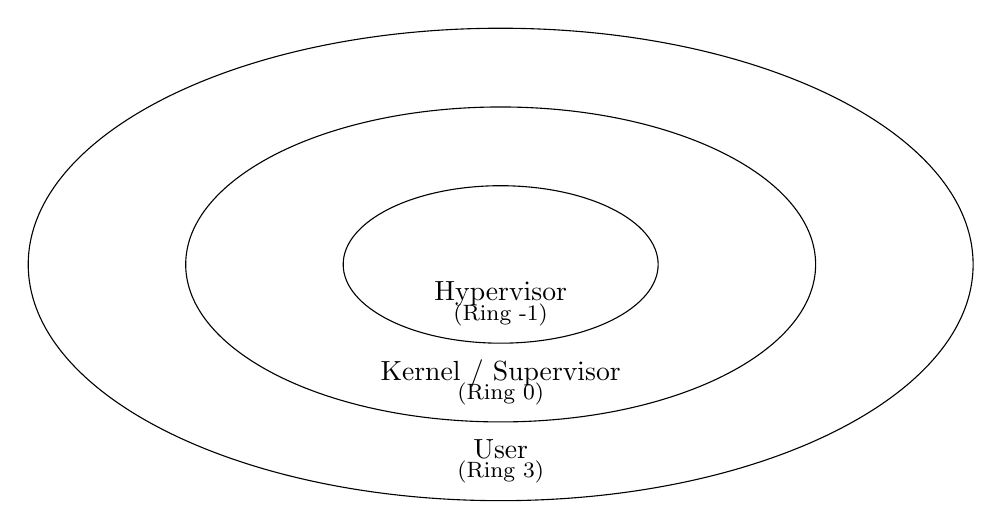
\begin{tikzpicture}
      \draw (0,0) ellipse (2cm and 1cm);
      \draw (0,0) ellipse (4cm and 2cm);
      \draw (0,0) ellipse (6cm and 3cm);
      \node [align=center] at (0, -0.5) {
        Hypervisor \\[-0.5em] \footnotesize (Ring -1)
      };
      \node [align=center] at (0, -1.5) {
        Kernel / Supervisor \\[-0.5em] \footnotesize (Ring 0)
      };
      \node [align=center] at (0, -2.5) {
        User \\[-0.5em] \footnotesize (Ring 3)
      };
    \end{tikzpicture}

    \begin{flushright}
      Each ring can access instructions in any of its outer rings
    \end{flushright}
  \end{frame}

  \begin{frame}
    \frametitle{The Kernel of the Operating System Runs in Kernel Mode}

    \begin{tikzpicture}
      \draw [primarycolor, dashed, thick] (0,0) -- ($(\textwidth - 3pt, 0)$);
      \node [primarycolor, anchor=south east] at ($(\textwidth - 3pt, 0)$)
            (user) {User space};
      \node [primarycolor, anchor=north east] at ($(\textwidth - 3pt, 0)$)
            (kernel) {Kernel space};
    \end{tikzpicture}
  \end{frame}

  \begin{frame}
    \frametitle{System Calls Transition between User and Kernel Mode}

    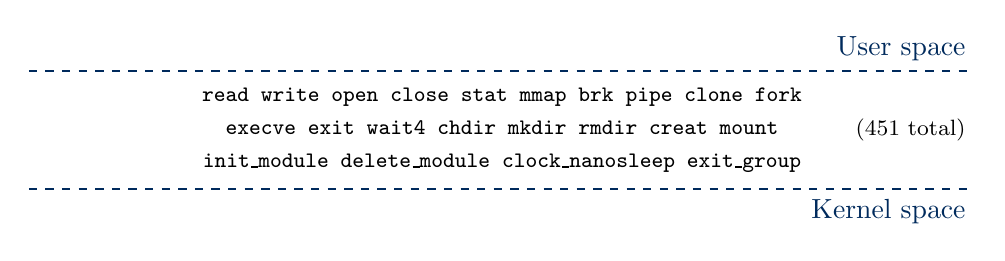
\begin{tikzpicture}
      \draw [primarycolor, dashed, thick] (0,0.75) -- ($(\textwidth - 3pt, 0.75)$);
      \node [primarycolor, anchor=south east] at ($(\textwidth - 3pt, 0.75)$)
            (user) {User space};
      \draw [primarycolor, dashed, thick] (0,-0.75) -- ($(\textwidth - 3pt, -0.75)$);
      \node [primarycolor, anchor=north east] at ($(\textwidth - 3pt, -0.75)$)
            (kernel) {Kernel space};
      \node [anchor=east] at ($(\textwidth - 3pt, -0)$) {\footnotesize (451 total)};
      \node [align=center] at ($(\textwidth/2 - 1.5pt, 0)$)
        {\footnotesize\ttfamily read write open close stat mmap brk pipe clone fork \\
         \footnotesize\ttfamily execve exit wait4 chdir  mkdir rmdir creat mount \\
         \footnotesize\ttfamily init\_module delete\_module clock\_nanosleep exit\_group };
    \end{tikzpicture}
  \end{frame}

  \begin{frame}
    \frametitle{System Calls Behave Like Regular Functions, But Run in Kernel
                Mode}

    \lstinline|ssize_t write(int fd, const void *buf, size_t count);|

    \vspace{1em}

    The \texttt{write} system call's API is:
    \begin{itemize}
      \item A file descriptor to write bytes to
      \item An address to contiguous sequence of bytes
      \item How many bytes to write from the sequence
    \end{itemize}
    
    \vspace{2em}

    \lstinline|void exit\_group(int status);|

    \vspace{1em}

    The \texttt{exit\_group} system call's API is:
    \begin{itemize}
      \item An exit code for the program (0-255)
    \end{itemize}

  \end{frame}

  \begin{frame}
    \frametitle{Let's Execute a 168 Byte ``Hello World'' on Linux AArch64}

    \scriptsize \ttfamily
    0x7F 0x45 0x4C 0x46 0x02 0x01 0x01 0x00 0x00 0x00 0x00 0x00 0x00 0x00 0x00
    0x00
    
    0x02 0x00 0xB7 0x00 0x01 0x00 0x00 0x00 0x78 0x00 0x01 0x00 0x00 0x00 0x00
    0x00
    
    0x40 0x00 0x00 0x00 0x00 0x00 0x00 0x00 0x00 0x00 0x00 0x00 0x00 0x00 0x00
    0x00
    
    0x00 0x00 0x00 0x00 0x40 0x00 0x38 0x00 0x01 0x00 0x40 0x00 0x00 0x00 0x00
    0x00
    
    0x01 0x00 0x00 0x00 0x05 0x00 0x00 0x00 0x00 0x00 0x00 0x00 0x00 0x00 0x00
    0x00
    
    0x00 0x00 0x01 0x00 0x00 0x00 0x00 0x00 0x00 0x00 0x01 0x00 0x00 0x00 0x00
    0x00
    
    0xA8 0x00 0x00 0x00 0x00 0x00 0x00 0x00 0xA8 0x00 0x00 0x00 0x00 0x00 0x00
    0x00
    
    0x00 0x10 0x00 0x00 0x00 0x00 0x00 0x00 0x08 0x08 0x80 0xD2 0x20 0x00 0x80
    0xD2
    
    0x81 0x13 0x80 0xD2 0x21 0x00 0xA0 0xF2 0x82 0x01 0x80 0xD2 0x01 0x00 0x00
    0xD4
    
    0xC8 0x0B 0x80 0xD2 0x00 0x00 0x80 0xD2 0x01 0x00 0x00 0xD4 0x48 0x65 0x6C
    0x6C
    
    0x6F 0x20 0x77 0x6F 0x72 0x6C 0x64 0x0A
  \end{frame}

  \begin{frame}
    \frametitle{ELF is the Binary Format for Unix Operating Systems}

    Executable and Linkable Format (ELF) is a file format

    \vspace{2em}

    Always starts with the 4 bytes: \hspace{0.5em} \texttt{0x7F 0x45 0x4C 0x46}

    \hspace{3em} or with ASCII encoding: \hspace{0.5em}
    \texttt{0x7F~~'E'~~'L'~~'F'}

    \vspace{2em}

    Followed by a byte signifying 32 or 64 bit architectures

    \hspace{2em} then a byte signifying little or big endian

    \vspace{4em}

    Most file formats have different starting signatures (or magic numbers)
  \end{frame}

  \begin{frame}
    \frametitle{Use \texttt{readelf} to Read ELF File Headers}

    Command: \hspace{0.5em} \texttt{readelf -a <filename>} (for all information)

    \vspace{1em}

    Contains the following:
    \begin{itemize}
      \item A header containing:
      \begin{itemize}
        \item Information about the machine (e.g. the ISA)
        \item The entry point of the program
      \end{itemize}
      \item Any \structure{program headers} (required for executables)
      \item Any \structure{section headers} (required for libraries)
    \end{itemize}
  \end{frame}

  \begin{frame}
    \frametitle{Our Minimal Executable Contains a Single Program Header}

    Tells the kernel to load the entire executable file into memory at
    address \texttt{0x10000}

    \vspace{2em}

    The header is 64 bytes, and the program header is 56 bytes (120 bytes total)

    \vspace{2em}

    The next 36 bytes are instructions, then 12 bytes for the string ``Hello
    world\textbackslash n''

    \vspace{1em}

    \hspace{2em} Instructions start at \texttt{0x10078} (\texttt{0x78} is 120)

    \vspace{1em}

    \hspace{2em} The string starts at \texttt{0x1009C} (\texttt{0x9C} is 156)
  \end{frame}


  \begin{frame}[fragile]
    \frametitle{``Hello world'' Needs 2 System Calls}

    Command: \hspace{0.5em} \texttt{strace <filename>}

    \vspace{2em}
    
    This shows all the system calls our program makes:

    \vspace{2em}

    \begin{lstlisting}[basicstyle=\scriptsize\ttfamily]
execve("./hello_world", ["./hello_world"], 0x7ffd0489de40 /* 46 vars */) = 0
write(1, "Hello world\n", 12)           = 12
exit_group(0)                           = ?
+++ exited with 0 +++
    \end{lstlisting}
  \end{frame}

  \begin{frame}
    \frametitle{Quick Aside: API Tells You What and ABI Tells You How} 

    Application Programming Interface (API) abstracts the details how how to
    communicate

    \vspace{2em}

    \hspace{2em} e.g. A function takes 2 integer arguments

    \vspace{4em}

    Application Binary Interface (ABI) specifies how to layout data and how to
    concretely communicate

    \vspace{2em}

    \hspace{2em} e.g. The same function using the C calling convention
  \end{frame}

  \begin{frame}
    \frametitle{System Call ABI for Linux AArch64}

    Enter the kernel with a \texttt{svc} instruction, using registers for
    arguments:

    \begin{itemize}
      \item \texttt{x8} --- System call number
      \item \texttt{x0} --- 1\textsuperscript{st} argument
      \item \texttt{x1} --- 2\textsuperscript{nd} argument
      \item \texttt{x2} --- 3\textsuperscript{rd} argument
      \item \texttt{x3} --- 4\textsuperscript{th} argument
      \item \texttt{x4} --- 5\textsuperscript{th} argument
      \item \texttt{x5} --- 6\textsuperscript{th} argument
    \end{itemize}

    What are the limitations of this?

    \vspace{2em}

    Note: other registers are not used, whether they're saved isn't important
    for us
  \end{frame}

  \begin{frame}[fragile]
    \frametitle{Instructions for ``Hello world'', Using the Linux AArch64 ABI}

    Plug in the next 36 bytes into a disassembler, such as:
    \url{https://onlinedisassembler.com/}

    \vspace{2em}

    Our disassembled instructions:
    \begin{lstlisting}[xleftmargin=2em]
mov x8, #0x40          // #64
mov x0, #0x1           // #1
mov x1, #0x9C          // #156
movk x1, #0x1, lsl #16 // #0x10000
mov x2, #0x0C          // #12
svc #0x0
mov x8, #0x5E          // #94
mov x0, #0x0           // #0
svc #0x0
    \end{lstlisting}
  \end{frame}

  \begin{frame}
    \frametitle{Finishing Up ``Hello world'' Example}

    The remaining 12 bytes is the ``Hello world'' string itself, ASCII encoded:
    
    \texttt{\footnotesize 0x48 0x65 0x6C 0x6C 0x6F 0x20 0x77 0x6F 0x72 0x6C 0x64 0x0A}

    \vspace{2em}

    \hspace{2em} Low level ASCII tip: bit 5 is \texttt{0}/\texttt{1} for upper
    case/lower case (values differ by 32)

    \vspace{2em}

    This accounts for every single byte of our 168 byte program, let's see what
    C does...

    \vspace{2em}
    Can you already spot a difference between strings in our example compared to
    C?
  \end{frame}

  \begin{frame}[fragile]
    \frametitle{Source Code for ``Hello world'' in C}

    \begin{lstlisting}
#include <stdio.h>

int main(int argc, char *argv[]) {
  printf("Hello world\n");
  return 0;
}
    \end{lstlisting}

    Compile with \lstinline|make| in \lstinline|lecture-02| in the examples
    repository

    \vspace{2em}

    What are other notable differences between this and our ``Hello world''?
  \end{frame}

  \begin{frame}[fragile]
    \frametitle{System Calls for ``Hello world'' in C, Finding Standard Library}
    \begin{lstlisting}[basicstyle=\ttfamily\scriptsize]
execve("./hello_world_c", ["./hello_world_c"], 0x7ffcb3444f60 /* 46 vars */) = 0
brk(NULL)                               = 0x5636ab9ea000
openat(AT_FDCWD, "/etc/ld.so.cache", O_RDONLY|O_CLOEXEC) = 3
fstat(3, {st_mode=S_IFREG|0644, st_size=149337, ...}) = 0
mmap(NULL, 149337, PROT_READ, MAP_PRIVATE, 3, 0) = 0x7f4d43846000
close(3)                                = 0
openat(AT_FDCWD, "/usr/lib/libc.so.6", O_RDONLY|O_CLOEXEC) = 3
read(3, "\177ELF\2\1\1\3\0\0\0\0\0\0\0\0\3\0>\0\1\0\0\0000C"..., 832) = 832
lseek(3, 792, SEEK_SET)                 = 792
read(3, "\4\0\0\0\24\0\0\0\3\0\0\0GNU\0\201\336\t\36\251c\324"..., 68) = 68
fstat(3, {st_mode=S_IFREG|0755, st_size=2136840, ...}) = 0
mmap(NULL, 8192, PROT_READ|PROT_WRITE, MAP_PRIVATE|MAP_ANONYMOUS, -1, 0)
  = 0x7f4d43844000
lseek(3, 792, SEEK_SET)                 = 792
read(3, "\4\0\0\0\24\0\0\0\3\0\0\0GNU\0\201\336\t\36\251c\324"..., 68) = 68
lseek(3, 864, SEEK_SET)                 = 864
read(3, "\4\0\0\0\20\0\0\0\5\0\0\0GNU\0\2\0\0\300\4\0\0\0\3\0\0", 32) = 32
    \end{lstlisting}
  \end{frame}

  \begin{frame}[fragile]
    \frametitle{System Calls for ``Hello world'' in C, Loading Standard Library}

    \begin{lstlisting}[basicstyle=\ttfamily\scriptsize]
mmap(NULL, 1848896, PROT_READ, MAP_PRIVATE|MAP_DENYWRITE, 3, 0) = 0x7f4d43680000
mprotect(0x7f4d436a2000, 1671168, PROT_NONE) = 0
mmap(0x7f4d436a2000, 1355776, PROT_READ|PROT_EXEC,
  MAP_PRIVATE|MAP_FIXED|MAP_DENYWRITE, 3, 0x22000) = 0x7f4d436a2000
mmap(0x7f4d437ed000, 311296, PROT_READ,
  MAP_PRIVATE|MAP_FIXED|MAP_DENYWRITE, 3, 0x16d000) = 0x7f4d437ed000
mmap(0x7f4d4383a000, 24576, PROT_READ|PROT_WRITE,
  MAP_PRIVATE|MAP_FIXED|MAP_DENYWRITE, 3, 0x1b9000) = 0x7f4d4383a000
mmap(0x7f4d43840000, 13888, PROT_READ|PROT_WRITE,
  MAP_PRIVATE|MAP_FIXED|MAP_ANONYMOUS, -1, 0) = 0x7f4d43840000
close(3)                                = 0
arch_prctl(ARCH_SET_FS, 0x7f4d43845500) = 0
mprotect(0x7f4d4383a000, 16384, PROT_READ) = 0
mprotect(0x5636a9abd000, 4096, PROT_READ) = 0
mprotect(0x7f4d43894000, 4096, PROT_READ) = 0
munmap(0x7f4d43846000, 149337)          = 0
fstat(1, {st_mode=S_IFCHR|0620, st_rdev=makedev(0x88, 0x1), ...}) = 0
    \end{lstlisting}
  \end{frame}

  \begin{frame}[fragile]
    \frametitle{System Calls for ``Hello world'' in C, Setting Up Heap and
                Printing}

    \begin{lstlisting}
brk(NULL)                               = 0x5636ab9ea000
brk(0x5636aba0b000)                     = 0x5636aba0b000
write(1, "Hello world\n", 12)           = 12
exit_group(0)                           = ?
+++ exited with 0 +++
    \end{lstlisting}

    \vspace{1em}
    The C version of ``Hello world'' ends with the exact same system calls we
    made
  \end{frame}

  \begin{frame}
    \frametitle{You Can Think of the Kernel as a Long Running Process}

    Writing kernel code is more like writing library code (there's no \texttt{main})

    \vspace{2em}

    The kernel lets you load code (called modules)

    \vspace{2em}

    Your code executes on-demand

    \hspace{2em} e.g. when it's loaded manually, new hardware, or accessing a certain file

    \vspace{2em}

    If you write a kernel module, you can execute privileged instructions

    \hspace{2em} and access any kernel data, so you could do anything
  \end{frame}

  \begin{frame}
    \frametitle{A Monolithic Kernel Runs Operating System Services in Kernel Mode}

    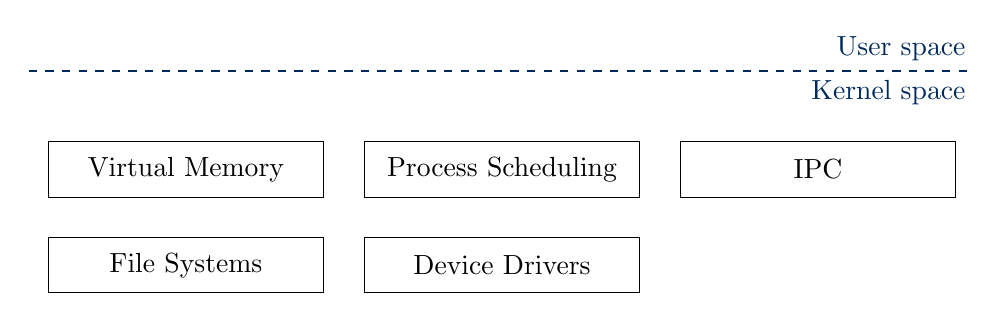
\begin{tikzpicture}[box/.style={draw, minimum width=3.5cm, minimum height=2em,
                                    inner sep=0.5em, node distance=0.5cm}]
      \draw [primarycolor, dashed, thick] (0,0) -- ($(\textwidth - 3pt, 0)$);
      \node [primarycolor, anchor=south east] at ($(\textwidth - 3pt, 0)$)
            (user) {User space};
      \node [primarycolor, anchor=north east] at ($(\textwidth - 3pt, 0)$)
            (kernel) {Kernel space};
      \node [box] (sched) at ($(\textwidth/2 - 1.5pt, -1.25)$) {Process Scheduling};
      \node [box, left=of sched] {Virtual Memory};
      \node [box, right=of sched] {IPC};
      \node [box, below=of sched] (dd) {Device Drivers};
      \node [box, left=of dd] {File Systems};
    \end{tikzpicture}
  \end{frame}

  \begin{frame}
    \frametitle{A Microkernel Runs the Minimum Amount of Services in Kernel Mode}

    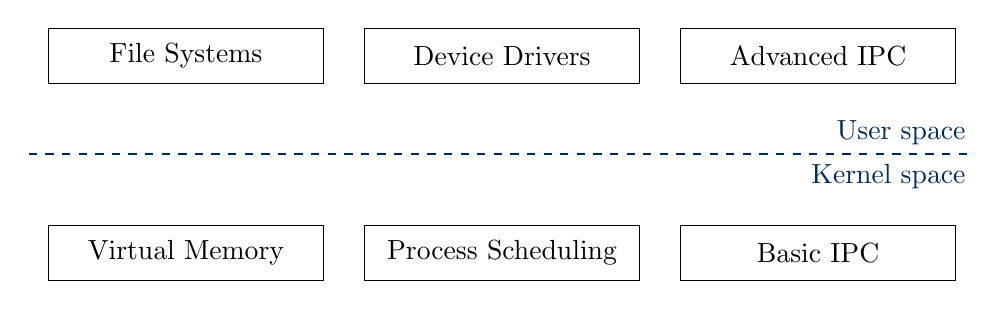
\begin{tikzpicture}[box/.style={draw, minimum width=3.5cm, minimum height=2em,
                                    inner sep=0.5em, node distance=0.5cm}]
      \draw [primarycolor, dashed, thick] (0,0) -- ($(\textwidth - 3pt, 0)$);
      \node [primarycolor, anchor=south east] at ($(\textwidth - 3pt, 0)$)
            (user) {User space};
      \node [primarycolor, anchor=north east] at ($(\textwidth - 3pt, 0)$)
            (kernel) {Kernel space};
      \node [box] (sched) at ($(\textwidth/2 - 1.5pt, -1.25)$) {Process Scheduling};
      \node [box, left=of sched] {Virtual Memory};
      \node [box, right=of sched] {Basic IPC};
      \node [box] (dd) at ($(\textwidth/2 - 1.5pt, 1.25)$) {Device Drivers};
      \node [box, left=of dd] {File Systems};
      \node [box, right=of dd] {Advanced IPC};
    \end{tikzpicture}
  \end{frame}

  \begin{frame}
    \frametitle{Other Types of Kernels}

    ``Hybrid'' kernels are between monolithic and microkernels

    \hspace{2em} Emulation services to user mode (Windows)

    \hspace{2em} Device drivers to user mode (macOS)

    \vspace{2em}

    Nanokernels and picokernels

    \hspace{2em} Move even more into user mode than traditional microkernels

    \vspace{4em}

    There's many different lines you can draw with different trade-offs
  \end{frame}

  \begin{frame}
    \frametitle{Kernel Interfaces Operate Between CPU Mode Boundaries}

    The lessons from the lecture:
    \begin{itemize}
      \item Code running in kernel mode is part of your kernel
      \item System calls are the interface between user and kernel mode
        \begin{itemize}
          \item Every program must use this interface!
        \end{itemize}
      \item File format and instructions to define a simple ``Hello world'' (in 168 bytes)
        \begin{itemize}
          \item Difference between API and ABI
          \item How to explore system calls
        \end{itemize}
      \item Different kernel architectures shift how much code runs in kernel mode
    \end{itemize}
  \end{frame}

\end{document}
